\section{Finding 9 - Credentials accessible inside container image}
\hrule
\begin{table}[htb]
    \renewcommand{\arraystretch}{1.5}
    \begin{tabular*}{\textwidth}{|>{\columncolor{red!15}}p{3cm}|p{17.2cm}|}
    \textbf{Finding} & \textbf{Credentials accessible inside container image}\\
    Risk& High\\
    Category& Information disclosure\\
    Impact& An attacker gains admin password of some service\\\\
    Description& Inside the container image of the previous finding insecure coding there was a 'cryptofs\_init' file. Opening the file there was a admin password as shown in the graphic below.
    \newline
    \newline
    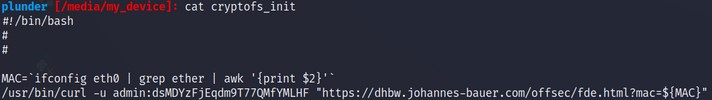
\includegraphics{cryptofs_init.jpg}
    \newline
	\\ 
    Recommendation& Credentials should be stored in a seperat environment. Further the password should not be stored in clear text in a file.\\
    \\\\\\\\\\\\\\\\\\\\\\\\\\\\\\\\ 
    \end{tabular*}
    \end{table}